\documentclass{article}

\usepackage{amsmath}
\usepackage{color}
\usepackage{listings}
\usepackage{xfrac}

\definecolor{dkgreen}{rgb}{0,0.6,0}
\definecolor{gray}{rgb}{0.5,0.5,0.5}
\definecolor{mauve}{rgb}{0.58,0,0.82}

\renewcommand{\thesubsection}{\alph{subsection}}
\renewcommand{\thesubsubsection}{\roman{subsubsection}}

\lstset{ %
  language=Python,                % the language of the code
  basicstyle=\footnotesize,           % the size of the fonts that are used for the code
  numbers=left,                   % where to put the line-numbers
  numberstyle=\tiny\color{gray},  % the style that is used for the line-numbers
  stepnumber=2,                   % the step between two line-numbers. If it's 1, each line 
                                  % will be numbered
  numbersep=5pt,                  % how far the line-numbers are from the code
  backgroundcolor=\color{white},      % choose the background color. You must add \usepackage{color}
  showspaces=false,               % show spaces adding particular underscores
  showstringspaces=false,         % underline spaces within strings
  showtabs=false,                 % show tabs within strings adding particular underscores
  frame=single,                   % adds a frame around the code
  rulecolor=\color{black},        % if not set, the frame-color may be changed on line-breaks within not-black text (e.g. commens (green here))
  tabsize=2,                      % sets default tabsize to 2 spaces
  captionpos=b,                   % sets the caption-position to bottom
  breaklines=true,                % sets automatic line breaking
  breakatwhitespace=true,        % sets if automatic breaks should only happen at whitespace
  title=\lstname,                   % show the filename of files included with \lstinputlisting;
                                  % also try caption instead of title
  keywordstyle=\color{blue},          % keyword style
  commentstyle=\color{dkgreen},       % comment style
  stringstyle=\color{mauve},         % string literal style
  escapeinside={\%*}{*)},            % if you want to add a comment within your code
  morekeywords={*,...}               % if you want to add more keywords to the set
}

\title{Problem Set 3}
\author{Alec Story \\ \small{avs38}}

\begin{document}
\maketitle

\section{}
\subsection{}
Since the mutation process is independent of the genealogical process, this is
equivalent to no mutation occuring on the path through the tree from one, to
their MRCA, and back down to the other.  Since we're ignoring the other
individuals in the sample, the time for this is just $2 \cdot T_{MRCA}$ for
$i=2$, which is equal to $2 \cdot T_2$, or 2.  Taking the number of mutations
$K$ as a Poisson random variable, we get
$$P\{K=0 | t=1\} = \frac{(\frac{\theta \cdot 2}{2})^0}{0!} \cdot
                   e^{-\frac{\theta \cdot 2}{2}}
                 = e ^{-\theta}$$

Extending this to the entire genealogy of n individuals is, then, the chance
that there is no mutation over the entire branch length of the tree.
$E[T_{Total}] = 2 \sum_{i=1}^{n-1} \frac{1}{i}$, so
\begin{align*}
 P\{K=0 | t = E[T_{Total}]) &= \frac{(\frac{
                               \theta 2 \sum_{i=1}^{n-1} \frac{1}{i}}{2})^0}{0!}
                               \cdot
                               e^{-\frac{
                               \theta 2 \sum_{i=1}^{n-1} \frac{1}{i}}{2}} \\
                            &= e^{-\theta \sum_{i=1}^{n-1} \frac{1}{i}}
\end{align*}
\subsection{}
The expected branch length between one sample and the MRCA is $T_{MRCA}$, and
its expectation is $2(1-\frac{1}{n})$.  Again taking mutations to be Poisson
distributed over that many generations, we get $E[K|t=2(1-\frac{1}{n})] =
\frac{\theta 2(1-\frac{1}{n})}{2} = \theta (1-\frac{1}{n})$
\section{}
For simplicity, we refer to the $n-1^\textrm{st}$ and $n-2^\textrm{nd}$
individuals as ``the mutants.''

Let $T_{R}$ be the time to the most recent common ancestor of the $n$ remainder
individuals.

Conceptually, we approach this problem by determining how much of the branch
length leading to the two mutants lies within the genealogy of the remainder
such that a mutation there would leave some of the remainder with one allele and
some with the other.  Since we are using the infinite sites model, only one
mutation at this locus can occur, so if we can determine the length $l$ of this
critical section, since we know the total length where the mutation could fall
($2 \cdot E[T_{MRCA}]$), the probability that the mutation spares the remainder is $1 -
\frac{l}{2 \cdot E[T_{MRCA}]}$.

First, consider the four cases that could lead the rest of the tree being
monomorphic:
\begin{description}
\item[a] Both mutants are outgroups to the remainder.  The probability of this
case is the probability that all the n individuals coalesce together before
coalescing with the mutants, $P(a) = \Pi_{i=1}^{n-1}\frac{n-1}{n+2-i}$.
\vspace{1in}

In this case, the critical section is entirely outside of the tree, so $l=0$.

\item[b] One mutant coalesces with the remainder at time $c$, and the other at
the MRCA of the entire sample.  This happens if the $n+1$ individuals including
one mutant coalesce together before the coalesce with the remaining mutant, but
not if they all coalesce first (case a), and since there are two ways to do this
we multiply by two to get $P(b) = 2 \Pi_{i=1}^n\frac{n-i}{n+2-i} - P(a)$.
\vspace{1in}

In this case, the critical section within the remainder's tree is of length $l =
T_R - c$.

\item[c] One mutant coalesces with the remainder at time $c_1$, and the other at
time $c_2$, and then they both coalesce at time $c_3$ where $c_1, c_2< c_3 < T_R$.
$P(c) = 1 - P(a) - P(b) - P(d)$.
\vspace{1in}

In this case, the critical section within the remainder's tree is of length $l =
(c_3 - c_1) + (c_3 - c_2)$.

\item[d] Both mutants coalesce with each other before they coalesce with the
remainder.  $P(d) = \frac{1}{n+1}$.
\vspace{1in}

In this case, the critical section is entirely outside the tree, so $l = 0$

Since these cases are independent, this leaves us to calculate the various
values we need:
\begin{align*}
E[T_{MRCA}] &= 2 ( 1 - \frac{1}{n+2}) \\
E[T_R] &= 2 ( 1 - \frac{1}{n}) \\
E[c] = E[c_1] = E[c_2] &= E[\textrm{Time of one lineage coalescing with n}] \\
                       &= \sum_{i=0}^{n-2} t(i)
                          (\frac{1}{n+1-i} + \frac{1}{n-i})\\
E[c_3] &= E[T_2] = 1 \\
\end{align*}

where $t(i)$ is the expected time of the $i^{\textrm{th}}$ coalescent event
(equivalently, the coalescent event when $n-i+1+1$ lineages are present),
which is equal to $\sum_{j=n-i+2}^{n+1} \frac{2}{j(j-1)}$.

Note that the sum in $E[c]$ is not up to $n-1$ because in the case where the sum
index reaches $n-1$, then we are considering the mutant coalescing \emph{after}
all the remainder coalesce, which we explicitly exclude from that part of the
probability space.

By independence, then, we get that
\begin{align*}
E[l] &= P(b) \cdot (E[T_R] - E[c]) + P(c) \cdot (2E[c_3] - E[c_1] - E[c_2]) \\
     &= P(b) \cdot (E[T_R] - E[c]) + P(c) \cdot (2E[c_3] - 2E[c_1])
\end{align*}

which does not simplify further on expansion, so I will leave it unsubstituted.
Recalling our first deductions, the final probability is $1 -
\frac{E[l]}{E[T_2]}$.

\end{description}

\section{}
\begin{align*}
E[K] &= \frac{\theta}{2} \cdot \{\textrm{The length of branches ancestral to
                                          all of a species}\} \\
     &= \frac{\theta}{2} \cdot (\tau + W_A - W_1 + \tau + W_A - W_2) \\
     &= \frac{\theta}{2} \cdot (2 \tau + 2 W_A - W_1 - W_2) \\
     &= \theta \cdot (\tau + W_A - \frac{W_1 + W_2}{2})
\end{align*}

\section{}
\subsection{}
Run on 100 individuals:

% GNUPLOT: LaTeX picture
\setlength{\unitlength}{0.240900pt}
\ifx\plotpoint\undefined\newsavebox{\plotpoint}\fi
\sbox{\plotpoint}{\rule[-0.200pt]{0.400pt}{0.400pt}}%
\begin{picture}(1500,900)(0,0)
\sbox{\plotpoint}{\rule[-0.200pt]{0.400pt}{0.400pt}}%
\put(191.0,131.0){\rule[-0.200pt]{4.818pt}{0.400pt}}
\put(171,131){\makebox(0,0)[r]{ 0}}
\put(1419.0,131.0){\rule[-0.200pt]{4.818pt}{0.400pt}}
\put(191.0,260.0){\rule[-0.200pt]{4.818pt}{0.400pt}}
\put(171,260){\makebox(0,0)[r]{ 500}}
\put(1419.0,260.0){\rule[-0.200pt]{4.818pt}{0.400pt}}
\put(191.0,389.0){\rule[-0.200pt]{4.818pt}{0.400pt}}
\put(171,389){\makebox(0,0)[r]{ 1000}}
\put(1419.0,389.0){\rule[-0.200pt]{4.818pt}{0.400pt}}
\put(191.0,518.0){\rule[-0.200pt]{4.818pt}{0.400pt}}
\put(171,518){\makebox(0,0)[r]{ 1500}}
\put(1419.0,518.0){\rule[-0.200pt]{4.818pt}{0.400pt}}
\put(191.0,647.0){\rule[-0.200pt]{4.818pt}{0.400pt}}
\put(171,647){\makebox(0,0)[r]{ 2000}}
\put(1419.0,647.0){\rule[-0.200pt]{4.818pt}{0.400pt}}
\put(191.0,776.0){\rule[-0.200pt]{4.818pt}{0.400pt}}
\put(171,776){\makebox(0,0)[r]{ 2500}}
\put(1419.0,776.0){\rule[-0.200pt]{4.818pt}{0.400pt}}
\put(191.0,131.0){\rule[-0.200pt]{0.400pt}{4.818pt}}
\put(191,90){\makebox(0,0){ 0}}
\put(191.0,756.0){\rule[-0.200pt]{0.400pt}{4.818pt}}
\put(347.0,131.0){\rule[-0.200pt]{0.400pt}{4.818pt}}
\put(347,90){\makebox(0,0){ 0.5}}
\put(347.0,756.0){\rule[-0.200pt]{0.400pt}{4.818pt}}
\put(503.0,131.0){\rule[-0.200pt]{0.400pt}{4.818pt}}
\put(503,90){\makebox(0,0){ 1}}
\put(503.0,756.0){\rule[-0.200pt]{0.400pt}{4.818pt}}
\put(659.0,131.0){\rule[-0.200pt]{0.400pt}{4.818pt}}
\put(659,90){\makebox(0,0){ 1.5}}
\put(659.0,756.0){\rule[-0.200pt]{0.400pt}{4.818pt}}
\put(815.0,131.0){\rule[-0.200pt]{0.400pt}{4.818pt}}
\put(815,90){\makebox(0,0){ 2}}
\put(815.0,756.0){\rule[-0.200pt]{0.400pt}{4.818pt}}
\put(971.0,131.0){\rule[-0.200pt]{0.400pt}{4.818pt}}
\put(971,90){\makebox(0,0){ 2.5}}
\put(971.0,756.0){\rule[-0.200pt]{0.400pt}{4.818pt}}
\put(1127.0,131.0){\rule[-0.200pt]{0.400pt}{4.818pt}}
\put(1127,90){\makebox(0,0){ 3}}
\put(1127.0,756.0){\rule[-0.200pt]{0.400pt}{4.818pt}}
\put(1283.0,131.0){\rule[-0.200pt]{0.400pt}{4.818pt}}
\put(1283,90){\makebox(0,0){ 3.5}}
\put(1283.0,756.0){\rule[-0.200pt]{0.400pt}{4.818pt}}
\put(1439.0,131.0){\rule[-0.200pt]{0.400pt}{4.818pt}}
\put(1439,90){\makebox(0,0){ 4}}
\put(1439.0,756.0){\rule[-0.200pt]{0.400pt}{4.818pt}}
\put(191.0,131.0){\rule[-0.200pt]{0.400pt}{155.380pt}}
\put(191.0,131.0){\rule[-0.200pt]{300.643pt}{0.400pt}}
\put(1439.0,131.0){\rule[-0.200pt]{0.400pt}{155.380pt}}
\put(191.0,776.0){\rule[-0.200pt]{300.643pt}{0.400pt}}
\put(30,453){\makebox(0,0){Count}}
\put(815,29){\makebox(0,0){T}}
\put(815,838){\makebox(0,0){Counts of Tij Aggregated by 0.1 Time Units}}
\put(191,246){\usebox{\plotpoint}}
\multiput(191.00,244.92)(0.534,-0.497){55}{\rule{0.528pt}{0.120pt}}
\multiput(191.00,245.17)(29.905,-29.000){2}{\rule{0.264pt}{0.400pt}}
\multiput(222.58,217.00)(0.497,2.424){59}{\rule{0.120pt}{2.023pt}}
\multiput(221.17,217.00)(31.000,144.802){2}{\rule{0.400pt}{1.011pt}}
\multiput(253.58,353.96)(0.497,-3.533){61}{\rule{0.120pt}{2.900pt}}
\multiput(252.17,359.98)(32.000,-217.981){2}{\rule{0.400pt}{1.450pt}}
\multiput(285.00,140.92)(1.439,-0.492){19}{\rule{1.227pt}{0.118pt}}
\multiput(285.00,141.17)(28.453,-11.000){2}{\rule{0.614pt}{0.400pt}}
\multiput(316.00,131.58)(0.499,0.497){59}{\rule{0.500pt}{0.120pt}}
\multiput(316.00,130.17)(29.962,31.000){2}{\rule{0.250pt}{0.400pt}}
\multiput(347.00,160.92)(0.499,-0.497){59}{\rule{0.500pt}{0.120pt}}
\multiput(347.00,161.17)(29.962,-31.000){2}{\rule{0.250pt}{0.400pt}}
\multiput(378.58,131.00)(0.497,1.576){59}{\rule{0.120pt}{1.352pt}}
\multiput(377.17,131.00)(31.000,94.195){2}{\rule{0.400pt}{0.676pt}}
\multiput(409.58,222.55)(0.497,-1.526){61}{\rule{0.120pt}{1.312pt}}
\multiput(408.17,225.28)(32.000,-94.276){2}{\rule{0.400pt}{0.656pt}}
\multiput(659.58,131.00)(0.497,1.364){59}{\rule{0.120pt}{1.184pt}}
\multiput(658.17,131.00)(31.000,81.543){2}{\rule{0.400pt}{0.592pt}}
\multiput(690.58,210.09)(0.497,-1.364){59}{\rule{0.120pt}{1.184pt}}
\multiput(689.17,212.54)(31.000,-81.543){2}{\rule{0.400pt}{0.592pt}}
\put(441.0,131.0){\rule[-0.200pt]{52.516pt}{0.400pt}}
\multiput(1377.58,131.00)(0.497,10.094){59}{\rule{0.120pt}{8.087pt}}
\multiput(1376.17,131.00)(31.000,602.215){2}{\rule{0.400pt}{4.044pt}}
\put(721.0,131.0){\rule[-0.200pt]{158.030pt}{0.400pt}}
\put(191.0,131.0){\rule[-0.200pt]{0.400pt}{155.380pt}}
\put(191.0,131.0){\rule[-0.200pt]{300.643pt}{0.400pt}}
\put(1439.0,131.0){\rule[-0.200pt]{0.400pt}{155.380pt}}
\put(191.0,776.0){\rule[-0.200pt]{300.643pt}{0.400pt}}
\end{picture}


This approximately matches the bimodal distribution we discussed in class, where
very high and very low pairwise differences dominate, as expected.
\subsection{}
The average $T_{MRCA}$ for 20 runs with a sample size of 100 and $t_0 = 0.3$ is
1.12.  This corresponds closely to the expected value calculated on the previous
problem set $2 - e^{-t_0/2} = 1.14$.
\subsection{}
\subsubsection{}
When run with 10 individuals and $\theta = 0.1$, most of the time, no mutations
occur.  Here is a (more interesting) run at $\theta = 10$:
\begin{verbatim}
0010000000010010100100
0000010010000100100100
0000000000000000100100
0001000000001000011011
0001000000001000011011
1000100000001000011011
0100001101100001000000
0000001101100001000000
0000001101100001000000
0000001101100001000000
\end{verbatim}
\subsubsection{}
\input{eta}
\section{}
\subsection{Constant Population Size}
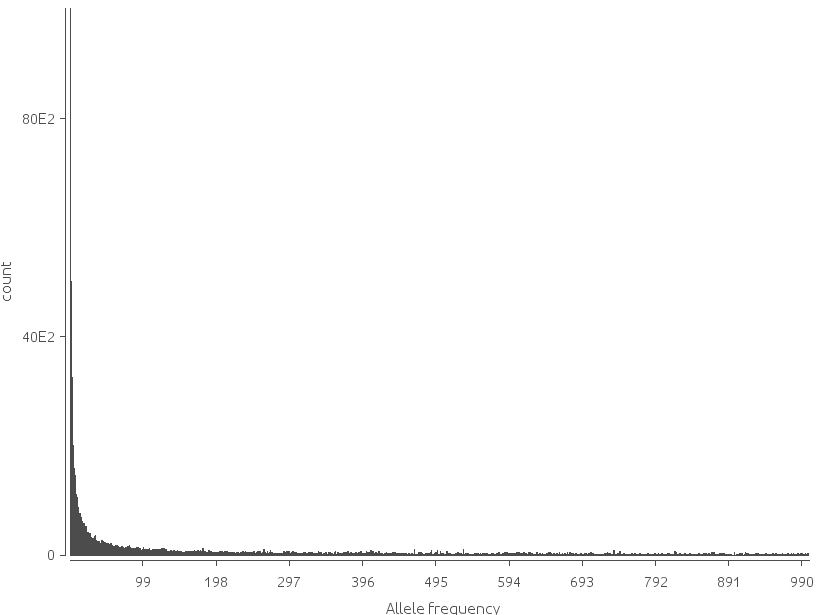
\includegraphics[width=\textwidth]{constant_size}
Tajima's D = -0.03756
\subsection{Growth at $\alpha = 100$}
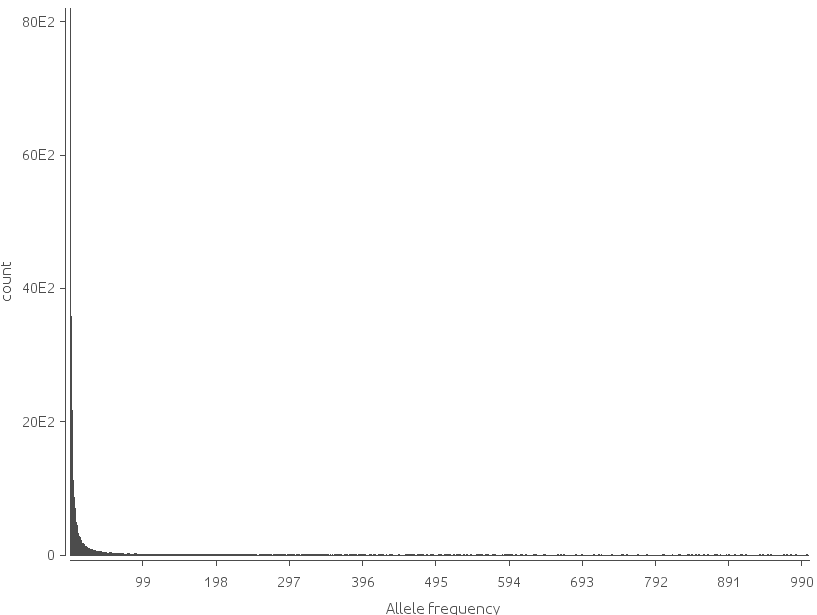
\includegraphics[width=\textwidth]{growth}
Tajima's D = -1.93785

Growth creates more alleles with low frequency because the genealogical tree has
more time towards the leaves than in the constant model, so there is more time
for mutations to occur that only affect a few individuals.  This also affects
Tajima's D by lowering it, since these mutations contribute little to the
pairwise differences while increasing the total number of segregating sites.
\subsection{Bottleneck at $t=0.3$}
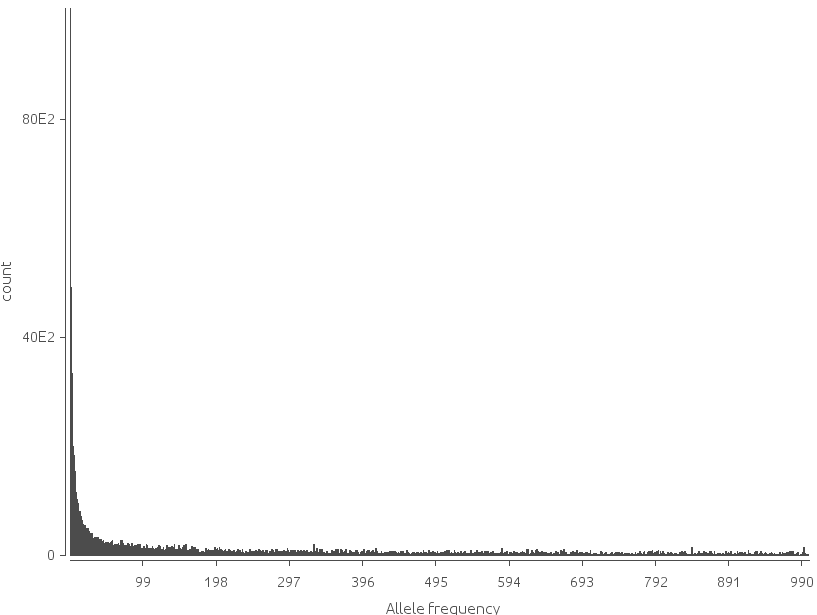
\includegraphics[width=\textwidth]{bottleneck}
Tajima's D = 0.58793

A bottleneck creates more alleles with high frequency because the alleles that
make it through the bottleneck are likely to remain at a high frequency
throughout the subsequent time.  This raises Tajima's D because these alleles
contribute highly to the pairwise differences.

\section{Code}
\subsection{coalescent.py}
\lstinputlisting[language=Python]{coalescent.py}
\subsection{lineage.py}
\lstinputlisting[language=Python]{lineage.py}

\end{document}
